\newpage
\subsection{Scrum}
\todo{The concept behind the Scrum approach is to empower the entire team to make
decisions, so that a project manager would become redundant. However, in order
to manage and make the best of the team's resources, the team found it
necessary to keep this position in this project.}

The Scrum approach is an iterative and incremental agile software development
framework that consists of three phases: The outline planning phase, which is
followed by a series of sprint cycles, and lastly a project closure phase.

These sprint cycles each consist of a single sprint, in which has a duration of
one to four weeks. Each sprint has three important parts: The first part is the
planning meeting, then the daily  meetings, and finally, the process is
concluded with an end meeting.
\begin{figure}[H]
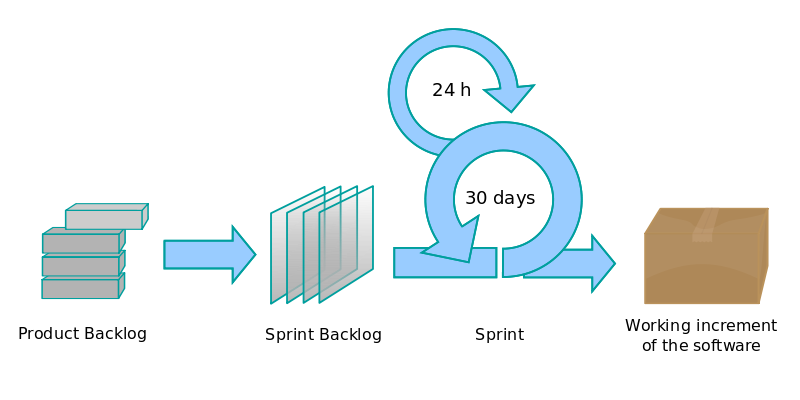
\includegraphics[width=\textwidth]{ch/projectManagement/fig/scrumProcess.png}
\caption{Illustration of the process in Scrum}
\end{figure}

\todo{refer to this illustration in the text}

\subsubsection{Sprint planning}
\label{sec:sprintplanning}
The objective of the sprint planning is to find out what work that needs to be completed within the duration of the sprint. This is done by preparing a sprint backlog that consists of the tasks to be done, called user stories. Each user story is estimated based on how much time the team thinks it will take to complete, based on previous experiences or lack of it, and difficulty level. In the Scrum approach, planning poker~\cite{planningpoker} is a common strategy to use for time planning.

\subsubsection{Planning poker}
In planning poker, each team member individually decide on how many units of time they think a task and/or user story will require to complete. This is repeated for each task and/or user story. The units of time can be in hours, work days, or whatever unit the team sees fit.

\todo{In the team's planning poker sessions, it was decided to use the units small (S), medium (M), large (L) and extra large (XL), each of them respectively representing one hour (S), two hours (M), four hours (L) and eight hours(XL).}

When a user story is presented, every team member presents the unit they believe the user story will require. If the entire team agrees on one estimate per user story, then the user story is assigned that particular estimate. If not, the team must discuss why they chose the particular unit and come to a conclusion the entire team agrees upon.
After this meeting the team should have a well prepared strategy for the sprint.

\todo{add illustration of planning poker}

\subsubsection{Daily meetings}
A work day is usually initiated with a daily meeting. The purpose of these meetings is to give an overview to the entire team of what all the other members are working on. For about fifteen minutes, all the team members briefly summarize which tasks they have performed and whether something went wrong.

By having this meeting, the team will quickly become aware if something has not gone as planned, such as a poorly estimated user story that requires more thought and replanning, or some other risk may occur, as discussed in section~\ref{sec:risk}. The result of having this meeting is that the problems that arise may be dealt with quickly.

\subsubsection{End meeting}
The end meeting is held at the end of a sprint. The meeting consists of a sprint review and a retrospective discussion for the last sprint.
Thus the project progress is reviewed, and accumulated lessons from the sprint can be taken in account for the next sprint.
It's also typical to have customer meetings to show what has been done so the customer can give feedback on whether or not he is satisfied with the product being developed.

\todo{bør denne være her? subsubsectionOur process
The team chose to have sprints with a duration of two weeks. Unfortunately, having daily meetings was not possible with the team's schedule. The team came to an agreement to meet twice a week, each beginning with a daily meeting. In addition, the team has a fixed time to meet with the customer once a week, unless the team or the customer does not see the need for it.}

\begin{comment}
\subsubsection{Scrum tool}
\label{sec:scrumtool}
The team has also decided to use a Scrum tool to make the process easier.
To find this tool, the team discussed what kind of functionality that would be useful to the project.

\todo[inline]{Add description from retrospect + add ref}
Specifically, the team wanted a tool that provided automatic sprint backlogs,
time measurements for each user story, graphs, and an interactive Scrum board.
%See section~\ref{sec:scrumtools} for further details.
\end{comment}
